\documentclass[12pt,twoside,a4paper]{book}
\usepackage[T1]{fontenc}
\usepackage[polish]{babel}
\usepackage[utf8]{inputenc}
\usepackage{graphicx}
\usepackage{enumitem}
\selectlanguage{polish}

%%%%% for titlepage from template %%%%%
\usepackage{amsmath}
\usepackage{graphicx}
\usepackage{parskip}
\usepackage{fancyhdr}
\usepackage{vmargin}
\setmarginsrb{3 cm}{2.5 cm}{3 cm}{2.5 cm}{1 cm}{1.5 cm}{1 cm}{1.5 cm}
\title{Opracowanie z Fizyki cz.1}
\author{Marcin Kamiński}
\date{Kwiecień 2017}
\makeatletter
\let\thetitle\@title
\let\theauthor\@author
\let\thedate\@date
\makeatother
\pagestyle{fancy}
\fancyhf{}
\rhead{\theauthor}
\lhead{\thetitle}
\cfoot{\thepage}

\begin{document}

%%%%%%%%%% TITLEPAGE %%%%%%%%%%
\begin{titlepage}
	\centering
	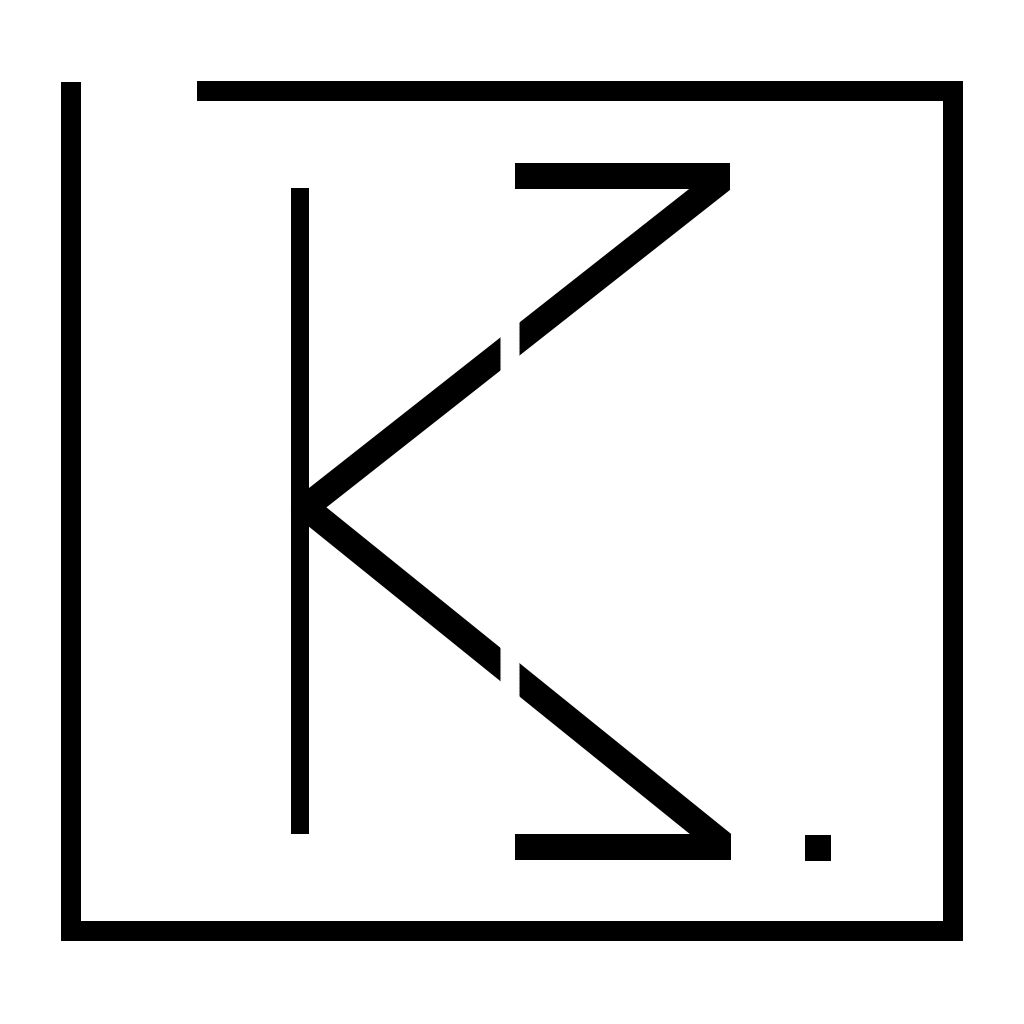
\includegraphics[scale = 0.1]{logo}\\[1.0 cm]	%LOGO
	\textsc{\Large Marcin Kamiński} %Author on frontPage
	\rule{\linewidth}{0.4 mm}
	\huge \bfseries {\thetitle}
	\rule{\linewidth}{0.4 mm}
	\textsc{\small \thedate}
\end{titlepage}


%%%%%%%%%% TABLE OF CONTENTS  %%%%%%%%%%
\raggedbottom
\tableofcontents


%%%%%%%%% MAIN %%%%%%%%%%
\chapter{Kinematyka}
Dział Fizyki zajmujący się opisem ruchu ciał (pomijający siły działające na ciała i przyczyny ruchu) nazywamy kinematyką.

\section{Ruch jednowymiarowy}
\begin{enumerate}[label=(\alph*)]
\item\textbf{Ruch} - \textit{zmiana położenia jednego ciała względem drugiego wraz z upływem czasu}
\item\textbf{Układ Odniesienia} - \textit{wybrane ciało lub układ ciał względem którego określamy położenie}
\item\textbf{Punkty materialne} - \textit{obiekty obdarzone masą, których rozmiary (objętość) mozemy zaniedbać}
\item\textbf{Prędkość} - \textit{zmiana pomożenia w jednostce czasu}
\item\textbf{Prędkość chwilowa} - \textit{zmiana położenia w bardzo małym przedziale czasu. Jest pochodną drogi względem czasu}
\item\textbf{Przyśpieszenie} - \textit{tempo zmian prędkości. Przyśpieszeniem chwilowym nazywamy pochodną prędkości po czasie}
\end{enumerate}

\section{Ruch na płaszczyźnie}
W układzie współrzędnych  ruch danego ciała możemy rozpatrywać jako wypadkową niezależnych ruchów wzdłóż różnych osi.
\begin{enumerate}[label=(\alph*)]
\item\textbf{Przemieszczenie} - \textit{odległość pomiędzy początkowym i końcowym położeniem ciała}
\item\textbf{Droga} - \textit{długość toru ruchu}
\item\textbf{Tor} - \textit{krzywa którą tworzą punkty płaszczyzny, przez które przechodzi poruszający się punkt materialny}
\item\textbf{Wektor prędkości} \textit{jest zawsze styczny do toru poruszającego się punktu, jest prostopadły do toru ruchu w ruchu po okręgu}
\item\textbf{Droga} - \textit{długość toru ruchu}
\item\textbf{Przyspieszenie styczne} - \textit{powoduje zmianę wartośći prędkości, ale nie zmienia kierunku i zwrotu}
\item\textbf{Przyspiesznie dośrodkowe} - \textit{występuje w ruchu po okręgu i jest skierowane w stronę środka okręgu, dla ruchu po dowolnej krzywej jest to przyspieszenie normalne lub radialne (skierowane wzdłuż promienia}
\item\textbf{Okres} - \textit{czas w którym punkt materialny wykona pełny obieg po okręgu}
\item\textbf{Przyspieszenie całkowite w ruchu krzywoliniowym} - \textit{suma przyspieszenia stycznego i przyspieszenia normalnego (ich sumą najczęściej jest skierowane pionowo w dół przyspieszenie grawitacyjne}
\end{enumerate}


\chapter{Dynamika}
Dynamika opisuje przyczyny ruchu.
\section{Podstawy dynamiki}
\begin{enumerate}[label=(\alph*)]
\item\textbf{Mechanika klasyczna} - \textit{zajmuje się rozpatrywaniem ruchu ciał poruszających się z małymi (w porównaniu z prędkością światła c) prędkościami}
\item\textbf{Droga} - \textit{długość toru ruchu}

\item Istnieją cztery podstawowe odddziaływania, z których wynikają wszystkie siły:
\begin{enumerate}[label=(\Roman*)]
\item\textbf{Oddziaływanie grawitacyjne} - \textit{siła grawitacyjna działa na wszystkie masy (jest siłą powszechną) i pochodzi od mas; ma długi zasięg i najmniejsze względne natężenie}
\item\textbf{Oddziaływanie elektromagnetyczne} - \textit{działa na ładunki i prądy, a jej źródłem są ładunki i prądy. Oddziaływanie elektromagnetyczne ma wielokrotnie większe natężenie od grawitacyjnego i długi zasięg}
\item\textbf{Oddziaływanie jądrowe}(silne) - \textit{utrzymuje w całości jądra atomowe pomimo
odpychania między protonami (ładunki dodatnie), ma bardzo krótki zasięg i największe
względne natężenie}
\item\textbf{Oddziaływanie słabe} - \textit{podlegają mu wszystkie cząstki elementarne,
w szczególności odpowiada za rozpady cząstek elementarnych}
\end{enumerate}
\item\textbf{Masa} - \textit{każdemu ciału przypisujemy masę, jeśli masa ciała zmienia się (jest nieznana w danej chwili) można wyznaczyć ją ze wzoru}
\item\textbf{Pęd} - \textit{iloczyn jego masy i prędkości (wektorowej)}
\item\textbf{Siła} - \textit{Jeżeli na ciało o masie m działa siła F, to definiujemy ją jako zmianę w czasie pędu tego ciała}
\item\textbf{Układ inercjalny} - \textit{Pierwsza zasada dynamiki stwierdza, że jeżeli na ciało nie działa żadna siła (lub gdy siła wypadkowa jest równa zeru) to istnieje taki układ odniesienia, w którym to ciało spoczywa lub porusza się ruchem jednostajnym prostoliniowym. Taki układ nazywamy układem inercjalnym. We wszystkich takich układach ruchami ciał rządzą dokładnie te sama prawa}
\item\textbf{Siła wypadkowa} - \textit{suma wszystkich sił działających na dane ciało}
\item\textbf{Siły wewnętrzne} - \textit{siły oddziaływania pomiędzy punktami materialnymi należącymi do danego układu}
\item\textbf{Siła zewnętrzna} - \textit{siły pochodzace spoza układu}
\item\textbf{Siły kontaktowe} - \textit{występują gdy dwa ciała stykają się (są dociskane do siebie). Źródłem tych sił jest odpychanie pomiędzy atomami. Przy dostatecznie małej odległości występuje
przekrywanie chmur elektronowych i ich odpychanie rosnące wraz z malejącą odległością.
Jest to siła elektromagnetyczna}
\item\textbf{Tarcie} - \textit{siła, która przeciwstawia się ruchowi, zawsze działa stycznie do powierzchni zetknięcia ciał i może istnieć nawet wówczas, gdy powierzchnie są nieruchome względem siebie. Siłę tarcia działającą między nieruchomymi powierzchniami nazywamy tarciem statycznym. $T_s$ jest w przybliżeniu niezależna od wielkości pola powierzchni styku ciał; $T_s$ jest proporcjonalna do siły z jaką jedna powierzchnia naciska na drugą. Tarcie kinetyczne wystepuje w momencie, w którym ciało się porusza. $T_k$ nie zależy od prędkości względnej poruszania się powierzchni}
\item\textbf{Układ nieinercjalny} - \textit{układ odniesienia poruszający się ruchem niejednostajnym względem jakiegokolwiek inercjalnego układu odniesienia}
\item\textbf{Siła bezwładności}(siła pozorna) - \textit{Iloczyn masy i przyspieszenia unoszenia (ze znakiem minus) nazywamy siłą bezwładności $F_b$, np. siła odśrodkowa}

\end{enumerate}
\section{Zasady dynamiki Newtona}
\begin{enumerate}[label=(\Roman*)]
\item\textit{Ciało, na które nie działa żadna siła (lub gdy siła wypadkowa jest równa zeru)
pozostaje w spoczynku lub porusza się ze stałą prędkością po linii prostej}
\item\textit{Jeżeli działająca na ciało siła wypadkowa jest różna od zera, to ciało porusza się z przyśpieszeniem, którego wartość jest wprost proporcjonalna do wartości siły wypadkowej działającej na to ciało i odwrotnie proporcjonalna do masy danego ciała\\
$$\vec a=\frac{\vec F}{m}$$\\
$\vec a$ - wektor przyspieszenia\\
$\vec F$ - wektor siły\\
$m$ - masa\\
\\W postaci uogólnionej: Tempo zmian pędu ciała jest równe sile wypadkowej działającej na to ciało. Dla
ciała o stałej masie sprowadza się to do iloczynu masy i przyspieszenia ciała}
\item\textit{Gdy dwa ciała oddziałują wzajemnie, to siła wywierana przez ciało drugie na ciało
pierwsze jest równa i przeciwnie skierowana do siły, jaką ciało pierwsze działa na
drugie}
\end{enumerate}
\section{Dodatkowe informacje}
\begin{enumerate}[label=(\alph*)]
\item\textbf{Siła Coriolisa} - \textit{powoduje odchylenie od linii prostej toru ruchu ciała, poruszającego się w układzie obracającym się (np. Ziemi lub płaskiej tarczy). Jest pozorna, występującą jedynie w obracających się układach nieinercjalnych}
\item\textbf{Przyspieszenie Coriolisa} - \textit{jest podwojonym iloczynem wektorowym prędkości kątowej i prędkości względnej}\\
$$\vec a_c = -2(\vec{\omega} \times \vec{v})$$\\
$\vec a_c$ \textit{- przyspieszenie Coriolisa}\\
$\vec{\omega}$ \textit{- prędkość kątowa układu}\\
$\vec{v}$ \textit{- prędkość ciała względem układu}\\

\end{enumerate}
\section{Grawitacja, prędkości kosmiczne}
\begin{enumerate}[label=(\alph*)]
\item\textbf{Prawo powszechnego ciążenia} - \textit{''Każde dwa ciała o masach $m_1$ i $m_2$ przyciągają się wzajemnie siłą grawitacji wprost proporcjonalną do iloczynu mas, a odwrotnie proporcjonalną do kwadratu odległości między nimi''}\\
$$\vec{F} = -G\frac{m_1 m_2}{r^2}\cdot\frac{\vec r}{r}$$\\
$\vec{F}$ - \textit{siła grawitacji}\\
$G$ - \textit{stała grawitacji}\\
$m_1$, $m_2$ - \textit{masy poszczególnych ciał punktowych lub kulistych}\\
$\vec r$ - wektor odległości między środkami ciał
\item\textit{Pierwsza prędkość kosmiczna to najmniejsza pozioma prędkość, jaką należy nadać ciału względem przyciągającego je ciała niebieskiego, aby ciało to poruszało się po zamkniętej orbicie. Z tak określonych warunków wynika, że dla ciała niebieskiego o kształcie kuli, orbita będzie orbitą kołową o promieniu równym promieniowi planety. Ciało staje się wtedy satelitą ciała niebieskiego}\\
$$v_I = \sqrt{\frac{GM}{R}}$$\\
$v_I$ - \textit{pierwsza prędkość kosmiczna}\\
$G$ - \textit{stała grawitacji}\\
$M$ - \textit{masa ciała niebieskiego, wokół którego orbituje dane ciało}\\
$R$ - \textit{odległość między środkami ciał}
\item\textit{Druga prędkość kosmiczna to prędkość, jaką należy nadać obiektowi, aby opuścił na zawsze dane ciało niebieskie, poruszając się dalej ruchem swobodnym. Inaczej – jest to prędkość, jaką trzeba nadać obiektowi na powierzchni tego ciała niebieskiego, aby tor jego ruchu stał się krzywą otwartą (parabolą lub hiperbolą). Obliczamy ją porównując energię obiektu znajdującego się na powierzchni ciała niebieskiego oraz w nieskończoności. Energia w nieskończoności równa jest 0 (zarówno energia kinetyczna jak i energia potencjalna pola grawitacyjnego), zatem na powierzchni sumaryczna energia też musi się równać 0}\\
$$v_{II} = \sqrt{\frac{2GM}{R}}$$
\item\textit{Trzecia prędkość kosmiczna to prędkość początkowa potrzebna do opuszczenia Układu Słonecznego}
\end{enumerate}
\section{Prawa Keplera}
\begin{enumerate}[label=(\Roman*)]
\item\textit{"Każda planeta układu słonecznego porusza się wokół Słońca po orbicie w kształcie elipsy, w której jednym z ognisk jest Słońce"} $a = -G \frac{G \cdot M \cdot m}{2U}$
\item\textit{"W równych odstępach czasu promień wodzący planety poprowadzony od Słońca, zakreśla równe pola"} $\overrightarrow{v_s} = \frac{d \overrightarrow{S}}{dt} = const$
\item\textit{"Stosunek kwadratu okresu obieu planety wokół Słońca do szcześcianu wielkiej półosi jej orbity (czyli średniej odległości od Słońca) jest stały dla wszystkich planet w układzie Słonecznym"} $\frac{T_1^2}{a_1^3} = \frac{T_2^2}{a_2^3} = const$
\end{enumerate}

\chapter{Praca, moc, energia, pęd}
\section{Praca}
\begin{enumerate}[label=(\alph*)]
\item\textbf{Praca} - \textit{wykonana przez stałą siłę F jest iloczynem skalarnym tej siły F i wektora
przesunięcia s. Dla siły zmiennej jest to pole pod wykresem (całka) siły, która wykonuje pracę (od $x_1$ do $x_2$}
\end{enumerate}

\section{Moc}
\begin{enumerate}[label=(\alph*)]
\item\textbf{Moc} - \textit{ilość wykonanej pracy (lub przekazanej energii) do czasu w jakim została ona wykonana. Jednostką mocy jest wat [W]}
\end{enumerate}

\section{Energia kinetyczna}
\begin{enumerate}[label=(\alph*)]
\item\textbf{Energia kinetyczna} - \textit{połowa iloczynu masy ciała i kwadratu prędkości}
\item\textbf{Praca} \textit{wykonana przez siłę F działającą na ciało o masie m jest równa zmianie
energii kinetycznej tego ciała. Jednostką pracy i energii jest dżul [J]}
\end{enumerate}

\section{Energia potencjalna}
\begin{enumerate}[label=(\alph*)]
\item\textbf{Energia potencjalna} - \textit{energia, jaką ma ciało lub układ ciał w zależności od położenia ciała (układu ciał) w przestrzeni. Pojęcie energii potencjalnej można wprowadzić jedynie wtedy, gdy ciało (układ ciał) oddziałuje z niezależnym od czasu polem sił potencjalnych}
\item\textit{Funkcję V(r) nazywamy potencjałem pola grawitacyjnego i definiujemy jako
stosunek grawitacyjnej energii potencjalnej masy m do wartości tej masy}
\end{enumerate}

\section{Zasada zachowania energii}
\begin{enumerate}[label=(\alph*)]
\item\textit{Zasada zachowania energii mechanicznej mówi, że dla ciała podlegającego działaniu siły zachowawczej, suma energii kinetycznej i potencjalnej jest stała. (Ta zasada jest bardziej ogólna i obowiązuje dla wszystkich odosobnionych układów ciał)}
\item\textit{Siła jest zachowawcza, jeżeli praca wykonana przez tę siłę nad punktem
materialnym, który porusza się po dowolnej drodze zamkniętej jest równa zeru}
\item\textit{Siła jest niezachowawcza jeżeli praca wykonana przez tę siłę nad punktem
materialnym, który porusza się po dowolnej drodze zamkniętej nie jest równa zeru}
\item\textit{Siłę nazywamy zachowawczą jeżeli praca wykonana przez nią nad punktem materialnym poruszającym się między dwoma punktami zależy tylko od tych punktów, a nie od łączącej je drogi. Siłę nazywamy niezachowawczą jeżeli praca wykonana przez nią nad punktem materialnym poruszającym się między dwoma punktami zależy od drogi łączącej te punkty}
\item\textit{Energia całkowita, tj. suma energii kinetycznej, energii potencjalnej i energii
wewnętrznej w układzie odosobnionym nie zmienia się. Mamy więc zasadę
zachowania energii całkowitej. Inaczej mówiąc energia może być przekształcana
z jednej formy w inną, ale nie może być wytwarzana ani niszczona; energia
całkowita jest wielkością stałą}
\end{enumerate}

\section{Zasada zachowania pędu}
\begin{enumerate}[label=(\alph*)]
\item\textbf{Środek masy} - \textit{jeden punkt, który porusza się po linii prostej ze stałą prędkością w danym układzie. Dla ciał o regularnym kształcie środek masy pokrywa się ze środkiem geometrycznym}
\item\textit{Środek masy układu punktów materialnych porusza się w taki sposób, jakby cała
masa układu była skupiona w środku masy i jakby wszystkie siły zewnętrzne nań działały}
\item\textit{Całkowity pęd układu punktów materialnych jest równy iloczynowi całkowitej masy
układu i prędkości jego środka masy}
\item\textbf{Zasada zachowania pędu - }\textit{Całkowity pęd układu punktów materialnych jest równy iloczynowi całkowitej masy układu i prędkości jego środka masy}
\end{enumerate}


\chapter{Zderzenia}
\section{Zderzenia}
\begin{enumerate}[label=(\alph*)]
\item\textbf{Siła impulsowa} - \textit{siła działająca przez bardzo krótki czas}
\item\textit{Gdy dwa ciała zderzają się to zderzenie może być sprężyste (elastyczne) lub
niesprężyste (nieelastyczne) w zależności od tego czy energia kinetyczna jest
zachowana podczas tego zderzenia czy też nie. Kiedy dwa ciała po zderzeniu łączą się mówimy, że zderzenie jest całkowicie niesprężyste}
\item\textbf{Zderzenie centralne} - \textit{zderzenie, które następuje gdy ciała poruszają się wzdłuż linii łączącej ich środki}
\item\textbf{Parametr zderzenia} - \textit{odległości między pierwotnym kierunkiem ruchu pierwszego ciała, a środkiem ciała spoczywającego}
\end{enumerate}
\section{Dodatkowe informacje}
\begin{enumerate}[label=(\alph*)]
\item\textbf{Siła ciągu} - \textit{siła będąca wynikiem działania silnika pojazdu, obiektu pływającego lub latającego}
\end{enumerate}

\chapter{Ruch Obrotowy}
\section{Kinematyka ruchu obrotowego}
\begin{enumerate}[label=(\alph*)]
\item\textbf{Przesunięcie kątowe} - \textit{wielkość analogiczna do przesunięcia w ruchu postępowym}
\item\textbf{Droga kątowa} - \textit{stosunek drogi liniowej i promienia}
\item\textbf{Prędkość kątowa} - \textit{tempo zmian drogi kątowej(pochodna drogi kątowej po czasie). Wielkość analogiczna do chwilowej prędkości liniowej}
\item\textbf{Przyspieszenie kątowe} - \textit{tempo zmian prędkości kątowej (pochodna prędkości kątowej po czasie)}
\end{enumerate}
\section{Dynamika ruchu obrotowego}
\begin{enumerate}[label=(\alph*)]
\item\textbf{(Wektor) Moment Siły} - \textit{jest wektorem osiowym (pseudowektorem), zaczepiony jest w punkcie O, a jego kierunek jest prostopadły do kierunku płaszczyzny wyznaczonej przez wektor F i promień wodzący r}
\item\textbf{Ramię Siły} - \textit{składowa siły która wpływa na jej wartość}
\item\textbf{Moment Pędu} - \textit{wektorowa wielkość fizyczna opisująca ruch (pęd) ciała, zwłaszcza jego ruch obrotowy}
\item\textbf{Moment bezwładności punktu materialnego} - \textit{iloczyn masy i kwadratu odległości od osi obrotu}
\item\textbf{Moment bezwładności bryły sztywnej} - \textit{Suma iloczynów masy i kwadratu odległości od osi obrotu poszczególnych punktów materialnych należących do danej bryły sztywnej}
\item\textbf{Pierwsza zasada dynamiki ruchu obrotowego} - \textit{,,Jeżeli na bryłę sztywną nie działają momenty sił lub działające momenty sił równoważą to bryła sztywna pozostaje w spoczynku lub porusza się ruchem obrotowym jednostajnym''}
\item\textbf{Druga zasada dynamiki ruchu obrotowego} - \textit{,,Jeżeli momenty sił działające na ciało nie równoważą się to bryła obraca się z przyspieszeniem kątowym $\epsilon$, którego wartość jest wprost proporcjonalna do wartości wypadkowego momentu siły, a odwrotnie proporcjonala do momentu bezwładności względem osi obrotu''}
\item\textbf{Duga zasada dynamiki dla ruchu obrotowego w postaci uogólnionej} -\textit{Wypadkowy moment siły działający na punkt materialny jest równy prędkości zmian momentu pędu w czasie }
\item\textbf{Trzecia zasada dynamiki ruchu obrotowego} - \textit{,,Jeżeli dwa ciała oddziałują wzajemnie, to moment sił z jakim działa ciało drugie na ciało pierwsze jest równy i przeciwnie skierowany do momentu siły, z jakim ciało pierwsze działa na drugie''}
\item\textbf{Zasada zachowania momentu pędu ruchu obrotowego} - \textit{,,Jeżeli na układ nie działa zewnętrzny moment siły (lub wypadkowy moment sił zewnętrznych jest równy zeru) to całkowity moment pędu układu pozostaje stały''}
\end{enumerate}
\section{Dynamika bryły sztywnej}
\begin{enumerate}[label=(\alph*)]
\item\textbf{Moment Bezwładności} - dla punktu materialnego jest to iloczyn masy i kwadratu odległości od osi obrotudanego ciała. Dla bryły jest to suma momentów bezwładności tych punktów materialnych.\textit{}
\end{enumerate}
\section{Ruch obrotowo postępowy}
\begin{enumerate}[label=(\alph*)]
\item\textit{Ruch ciała będący złożeniem ruchu postępowego środka masy i obrotowego
względem osi przechodzącej przez środek masy jest równoważny ruchowi
obrotowemu wokół osi przechodzącej przez punkt styczności ciała z powierzchnią,
po której się ono toczy}
\end{enumerate}

\chapter{Ruch drgający}
Ruch, który powtarza się w regularnych odstępach czasu, nazywamy ruchem okresowym.
\section{Siła sprężystości, drgania swobodne}
\begin{enumerate}[label=(\alph*)]
\item\textbf{Siła sprężystości (harmoniczna)} - \textit{siła działająca na ciało proporcjonalną
do przesunięcia tego ciała od początku układu i skierowaną ku początkowi układu}
\item\textbf{Drgania swobodne} - \textit{drgania, gdy siła sprężystości jest zarazem siłą wypadkową nazywamy}
\item\textbf{Amplituda} - \textit{maksymalne odchylenie}
\item\textbf{Faza drgań} - \textit{dzieli się na np. fazę początkową}
\item\textbf{Wahadło proste} - \textit{wyidealizowane ciało o masie punktowej,
zawieszone na cienkiej, nieważkiej, nierozciągliwej nici}
\item\textbf{Wahadło fizyczne} - \textit{ciało sztywne zawieszone tak, że może się wahać
wokół pewnej osi przechodzącej przez to ciało}
\item\textbf{Stała czasowa} - \textit{$\tau = m / \gamma$}
\item\textbf{Częstość własna} - \textit{(częstość drgań nietłumionych)  $\omega_{0} = \sqrt{k/m}$}
\end{enumerate}
\section{Oscylator harmoniczny tłumiony i drgania wymuszone}
\begin{enumerate}[label=(\alph*)]
\item\textbf{Współczynnik tłumienia} - \textit{określa wielkość tłumienia  $\beta = \sqrt{1/2 \tau}$, wpływa na czynnik tłumiący $e^{-\beta t}$
\item\textbf{Słabe tłumienie} - \textit{dla $\beta_{0} < \omega_{0}$ występuje słabe tłumienie, wtedy istnieje możliwość, że pomimo strat energii zachowany zostaje oscylacyjny charakter ruchu ($\omega = \sqrt{\omega_{0}^2-\beta^2}$})}
\item\textbf{Ruch pełzający (aperiodyczny)} - \textit{występuje gdy współczynnik tłumienia jest większy od początkowej częstości drgań $\beta > \omega_{0}$ (bardzo duża siła tłumiąca). Dzieje się tak na przykład gdy ruch odbywa się w bardzo gęstym ośrodku.}
\item\textbf{Tłumienie krytyczne} - \textit{występuje w szczególnej sytuacji gdy $\beta = \omega_{0}$}
\item\textbf{Współczynnik dobroci} - \textit{za jego pomocą opisywane są straty energii wynikające z tłumienia}
\item\textbf{Siła wymuszająca} - \textit{siła zewnętrzna przyłożona do oscylatora podtrzymująca drgania. W przypadku drgań harmonicznych zewnętrzna siła wymuszająca jest siłą okresowo zmienną}
\item\textit{Gdy układ jest zasilany współczynnikiem tłumienia $\beta$ relacją z częstością $\omega$ różną od częstości własnej $\omega_{0}$. W takiej sytuacji drgania (wymuszone) odbywają się z częstością siły zewnętrznej, a nie z częstością własną.}
\item\textbf{Rezonans} - \textit{zjawisko zachodzące dla drgań wymuszonych, objawiające się wzrostem amplitudy drgań układu 
drgającego dla określonej częstotliwości siły wymuszającej}
\item\textbf{Częstotliwość(amplituda) rezonansowa} - \textit{częstotliwość, dla której drgania mają największą amplitudę}
\item\textbf{Częstość rezonansowa} - \textit{wartości częstości siły wymuszającej dla której amplituda drgań jest maksymalna}
\end{enumerate}
\section{Składanie drgań harmonicznych (równoległych i prostopadłych)}
\begin{enumerate}[label=(\alph*)]
\item\textbf{Drgania przesunięte w fazie} - \textit{drgania przesunięte w czasie, ale odbywające się z jednakową częstotliwością}
\item\textbf{Superpozycja drgań} - \textit{zasada dodawania przemieszczeń drgań równoległych. Dla drgań odbywających się niezależnie przemieszczenie punktu materialnego jest sumą przemieszczeń składowych}
\end{enumerate}

\chapter{Fale w ośrodkach sprężystych}
\section{Fale mechaniczne}
\begin{enumerate}[label=(\alph*)]
\item\textbf{Ruch falowy} - \textit{rozchodzenie się zaburzenia w ośrodku. Właściwości sprężyste ośrodka decydują o prędkości rozchodzenia się fali}
\item\textbf{Energia fal} - \textit{energia kinetyczna i potencjalna cząstek ośrodka}
\item\textbf{Fale podłużne} - \textit{gdy kierunek drgań cząstek ośrodka jest równoległy do kierunku
rozchodzenia się fali i zarazem kierunku transportu energii, np. fale dźwiękowe w powietrzu}
\item\textbf{Fale poprzeczne} - \textit{gdy kierunek drgań cząstek ośrodka jest prostopadły do kierunku
rozchodzenia się fali i zarazem kierunku transportu energii, np. drgania naprężonego sznura, którego końcem poruszamy cyklicznie w górę i w dół}
\item\textbf{Impuls falowy} - \textit{powstaje gdy źródłem jest jednorazowe zaburzenie w ośrodku: na przykład
gdy wrzucimy kamień do wody lub gdy jednorazowo odchylimy koniec napiętej liny}
\item\textbf{Fala harmoniczna} - \textit{powstaje gdy źródło wykonuje drgania harmoniczne: na przykład gdy
cyklicznie wychylamy koniec napiętej liny}
\item\textbf{Czoło fali (powierzchnia falowa)} - \textit{powierzchnię łączącą punkty, do których w danej chwili dotarła fala}
\item\textbf{Promień fali} - \textit{linia prosta, prostopadła do czoła fali, wskazującą kierunek ruchu fali}
\item\textbf{Fala płaska} - \textit{zaburzenie rozchodzi się w jednym kierunku, a powierzchnie
falowe są płaszczyznami prostopadłymi do kierunku ruchu fali}
\item\textbf{Fala kulista} - \textit{zaburzenie rozchodzi się ze źródła we wszystkich kierunkach,
a powierzchnie falowe są sferami}
\item\textbf{Amplituda fal} - \textit{maksymalne wychylenie}
\item\textbf{Faza} - \textit{wybrana część fali (w pewnym momencie)}
\item\textbf{Długość fali} - \textit{odległość między punktami o tej samej fazie na przykład między dwoma grzbietami (maksimami)}
\item\textbf{Okres (T)} - \textit{czas, w którym fala przebiega odległość równą $\lambda$}
\item\textbf{Prędkość fazowa} - \textit{prędkość fali dla wybranej fazy}
\item\textbf{Prędkość grupowa} - \textit{w przypadku gdy zaburzenie falowe jest złożeniem fal sinusoidalnych o różnych
częstotliwościach to prędkość przenoszenia energii (prędkość fali modulowanej) może być
inna niż prędkości fal składowych}
\item\textbf{Interferencja fal} - \textit{zjawisko nakładania się fal}
\item\textbf{Fala stojąca} - \textit{fala której cząstki ośrodka drgają ruchem harmonicznym prostym ale w przeciwieństwie do fali bieżącej różne punkty ośrodka mają różną amplitudę drgań zależną od ich położenia $x$}
\item\textbf{Strzałki} - \textit{punkty o największej amplitudzie}
\item\textbf{Węzły} - \textit{punkty nie wykonujące drgań (mające zerową aplitudę)}
\end{enumerate}
\section{Analiza fal złożonych, dudnienia, modulacja amplitudy, zjawisko Dopplerra}
\begin{enumerate}[label=(\alph*)]
\item\textbf{Częstość podstawowa} - \textit{najniższa częstość}
\item\textbf{Alikwoty} - \textit{tzw. wyższe harmoniczne, tzn. częstości różne od częstości podstawowych}
\item\textit{Dowolne drganie okresowe o okresie T możemy przedstawić jako kombinację liniową (sumę) drgań harmonicznych o okresach danych wzorem $T_n = T/n$, gdzie n jest liczbą naturalną}
\item\textbf{Modulacja Amplitudy (AM)} - \textit{występuje gdy częstotliwości $f_1$ i $f_2$ są bliskie siebie to amplituda zmienia się powoli $(f_{amp.}$ jest mała)}
\item\textbf{Zjawisko Dopplera} - \textit{polega na pozornej zmianie częstotliwości fali z powodu ruchu
obserwatora lub źródła fali}
\end{enumerate}

\chapter{Statyka i dynamika płynów}
Mówimy, że płyny nie mają \textit{sprężystości kształtu}, a mają \textit{sprężystość objętości}. Dlatego rozwiązanie
zagadnień z mechaniki płynów wymaga posługiwania się pojęciami takimi jak ciśnienie i gęstość.
\section{Ciśnienie i gęstość}
\begin{enumerate}[label=(\alph*)]
\item\textbf{Siła parcia} - \textit{siła powierzchniowa w cieczy, jest zawsze prostopadła do powierzchni płynu podczas gdy w ciele stałym może mieć dowolny kierunek. Spoczywający płyn nie może równoważyć sił stycznych (warstwy
płynu ślizgałyby się po sobie) i dlatego może zmieniać kształt i płynąć.}
\item\textbf{Ciśnienie} - \textit{stosunek siły parcia działającej na jednostkę powierzchni
do wielkości tej powierzchni}
\item\textit{Długość wektora S jest równa polu powierzchni S, jego kierunek jest prostopadły do
powierzchni, a zwrot na zewnątrz powierzchni.}
\item\textbf{Gęstość} - \textit{stosunek masy pewnej (ilości) substancji do zajmowanej przez nią objętości}
\item\textbf{Ciężar właściwy} - \textit{ciężar warstwy płynu leżącej pomiędzy punktami, dla których mierzymy różnicę ciśnień}
\item\textbf{Prawo Pascala} - \textit{"Ciśnienie zewnętrzne wywierane na zamknięty płyn jest przekazywane niezmienione
na każdą część płynu oraz na ścianki naczynia"}
\item\textbf{Prawo Archimedesa} - \textit{"Ciało w całości lub częściowo zanurzone w płynie jest wypierane ku górze siłą równą ciężarowi wypartego przez to ciało płynu"}
\item\textbf{Siła wyporu} - \textit{siła, którą wywiera ciecz na każdą, będącą z nią w kontakcie, część powierzchni ciała które jest częściowo lub całkowicie w niej zanurzone}
\item\textbf{Przepływ ustalony(laminarny) lub nieustalony} - \textit{ruch płynu jest
ustalony, gdy prędkość płynu v w dowolnie wybranym punkcie jest stała w czasie tzn.
każda cząsteczka przechodząca przez dany punkt zachowuje się tak samo. Warunki takie
osiąga się przy niskich prędkościach przepływu}
\item\textbf{Przepływ wirowy lub bezwirowy} - \textit{przepływ jest bezwirowy, gdy
w żadnym punkcie cząsteczka nie ma wypadkowej prędkości kątowej}
\item\textbf{Przepływ ściśliwy lub nieściśliwy} - \textit{przepływ jest nieściśliwy gdy gęstość
płynu jest stała. Zazwyczaj przepływ cieczy jest nieściśliwy. Również przepływ gazu
może być w pewnych warunkach nieściśliwy. Przykładem może tu być ruch powietrza
względem skrzydeł samolotu podczas lotu z prędkością mniejszą od prędkości dźwięku}
\item\textbf{Przepływ lepki lub nielepki} - \textit{lepkość w ruchu płynów jest
odpowiednikiem tarcia w ruchu ciał stałych. Charakteryzuje opór płynów przeciw
płynięciu pod działaniem sił zewnętrznych. Lepkość jest istotną cechą wielu produktów
na przykład smarów}
\item\textbf{Linia prądu} - \textit{tor jednej cząstki(a tym samym tor każdej cząstki) przechodzącej przez dany punkt}
\item\textbf{Struga prądu} - \textit{pewną skończona liczba linii prądu}
\item\textit{Prędkość płynu nieściśliwego przy ustalonym przepływie jest odwrotnie
proporcjonalna do pola przekroju strugi, co wynika z równania ciągłości}
\item\textbf{Równanie(Prawo) Bernoulliego} - \textit{Suma ciśnień statycznego i dynamicznego w cieczy lub gazie jest stała w czasie ich przepływu \\ $e_m = \frac{v^2}{2} + gh + \frac{p}{\rho} = const$}
\item\textit{W odróżnieniu od statycznej siły nośnej , którą jest siła wyporu działającą zgodnie
z prawem Archimedesa na przykład na balon czy statek, dynamiczna siła nośna
wywołana jest ruchem ciał w płynie, na przykład na skrzydła samolotu czy śmigła
helikoptera.}
\end{enumerate}

\chapter{Dodatkowe}
\begin{enumerate}[label=(\alph*)]
\item\textbf{Przemiana izobaryczna}: \textit{$p=const$ $W=p \Delta V$ , $const=\frac{v}{T}$, $\Delta Q = m \cdot c_p \Delta T$}
\item\textbf{Przemiana izochoryczna}: \textit{$V=const, \frac{p_1}{T_1}=\frac{p_2}{T_2}=const, W=p\Delta V=0, \Delta U=Q=mc_v(T_2-T_1)$}
\item\textbf{Przemiana Izotermiczna}: \textit{$T=const, pV=const, \Delta U =mc_v\Delta T=0, Q=W=RTln\frac{v_2}{v_1} $}
\item\textbf{Przemiana Adiabatyczna}: \textit{$pV^k=const, k=\frac{C_p}{C_v}, \Delta U=-W, W=mc\Delta T, \Delta Q=0 $}
\end{enumerate}
\begin{center}
\label{Jednostki}
\begin{figure}
\caption{Jednostki układu SI}
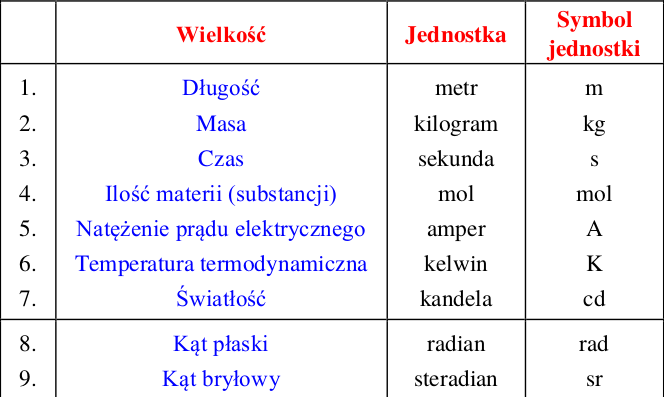
\includegraphics[width=\textwidth]{graphics/1}
\end{figure}

\vspace{1cm}
\begin{figure}
\caption{Skróty}
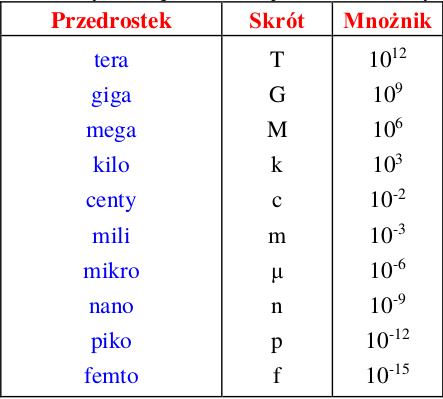
\includegraphics[width=\textwidth]{graphics/2}
\end{figure}

\vspace{1cm}
\begin{figure}
\caption{Wyznaczanie kierunku wektora (zasada prawej ręki)}
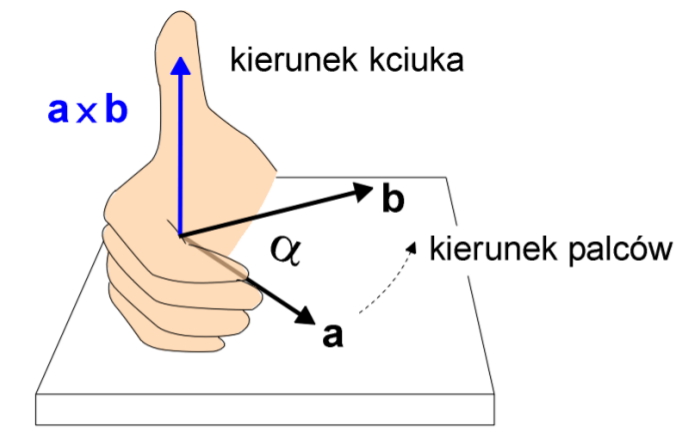
\includegraphics[width=\textwidth]{graphics/3}
\end{figure}

\vspace{1cm}
\begin{figure}
\caption{Analiza rzutu ukośnego}
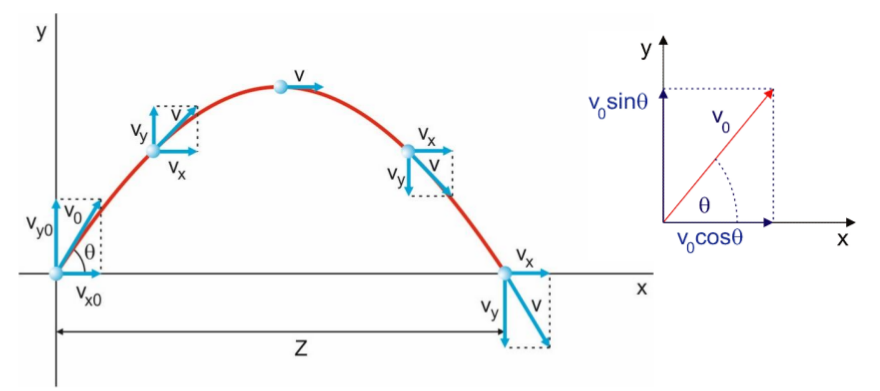
\includegraphics[width=\textwidth]{graphics/4}
\end{figure}

\vspace{1cm}
\begin{figure}
\caption{Analiza ruchu po okręgu}
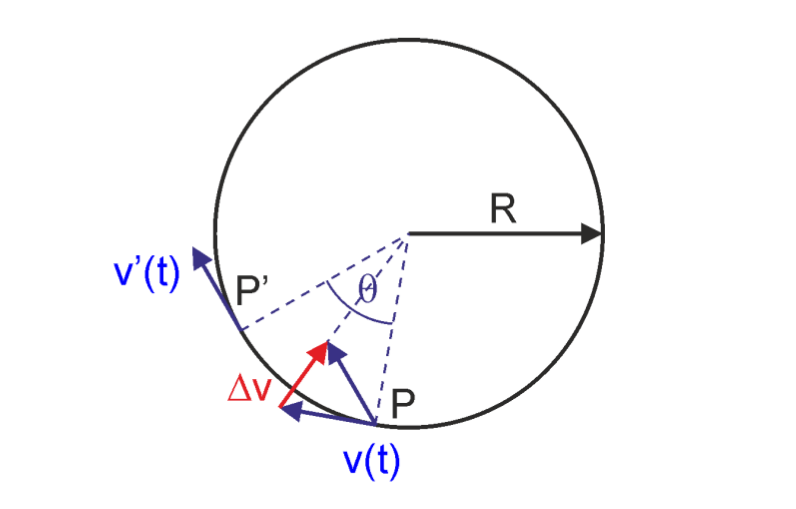
\includegraphics[width=\textwidth]{graphics/5}
\end{figure}

\vspace{1cm}
\begin{figure}
\caption{Oddziaływania}
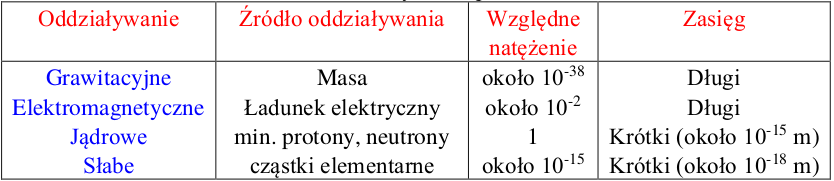
\includegraphics[width=\textwidth]{graphics/6}
\end{figure}
\end{center}

\chapter{Wzory}
\textit\small{{x - przemieszczenie/położenie,  v - prędkość, s - droga, a - przyspieszenie, t - czas, h - wysokość, z - zasięg, p - pęd, W - praca, F - siła, E - energia, g - przyspieszenie ziemskie, P - moc, p - ciśnienie, T - siła tarcia, $\rho$ - gęstość, M - moment siły, L - moment pędu, I - moment bezwładności, $\omega$ - prędkość kątowa, $\epsilon$ - przyspieszenie kątowe, G - stała grawitacyjna, }}
\section{Wektory}
\begin{enumerate}
\item$(\overrightarrow{a}x\overrightarrow{b})x\overrightarrow{c}=\overrightarrow{b}(\overrightarrow{a}o\overrightarrow{c})-\overrightarrow{c}(\overrightarrow{a}o\overrightarrow{b})$
\item$|\overrightarrow{a}x\overrightarrow{b}|=|\overrightarrow{w}|=\sqrt{(w_{x})^2+(w_{y})^2+(w_{z})^2}$
\item$\overrightarrow{a}x\overrightarrow{b}=|\overrightarrow{a}|\cdot|\overrightarrow{b}|\cdot sin\alpha=det[\overrightarrow{a}x\overrightarrow{b}]$
\item$\overrightarrow{a}o\overrightarrow{b}=|\overrightarrow{a}|\cdot|\overrightarrow{b}|\cdot cos\alpha$
\end{enumerate}
\section{Kinematyka}
\begin{enumerate}
\item$\overrightarrow{v} = \frac{\overrightarrow{x}}{t}$
\item$\overrightarrow{v_{ch}} = \frac{d\overrightarrow{x}}{dt}$
\item$\overrightarrow{v_{sr}} = \frac{\Delta \overrightarrow{x}}{\Delta t}$
\item$v=\frac{s}{\Delta t}$
\item$\overrightarrow{a} = \frac{\overrightarrow{v}}{t}$
\item$\overrightarrow{a_{ch}} = \frac{d\overrightarrow{v}}{dt}$
\item$\overrightarrow{a_{sr}} = \frac{\Delta \overrightarrow{v}}{\Delta t}$
\item$v_{x}= a_{x_0} \cdot t$
\item$v_{y}= -g \cdot t$
\item$x(t)= v_{x_0} \cdot t$
\item$y(t)= h - \frac{g \cdot t^2 }{2} - v_0 \cdot t$
\item$\overrightarrow{v_o} = \overrightarrow{v_x} + \overrightarrow{v_y}$
\item$h_{max} = \frac{(2 \cdot v_0 \cdot sin\alpha)^2}{2 \cdot g}$
\item$z = \frac{(v_0)^2}{g} \cdot sin2\alpha$
\item$W = \int_{x_0}^{x} Fdx$
\item$p = mv$
\item$E_k = \frac{mv^2}{2} = \frac{p \cdot v}{2}$
\end{enumerate}
\section{Dynamika}
\begin{enumerate}
\item$\overrightarrow{v} = \frac{\overrightarrow{x}}{t}$
\item$\overrightarrow{v_{ch}} = \frac{d\overrightarrow{x}}{dt}$
\item$\overrightarrow{v_{sr}} = \frac{\Delta \overrightarrow{x}}{\Delta t}$
\item$v=\frac{s}{\Delta t}$
\item$v_{x}= a_{x_0} \cdot t$
\item$v_{y}= -g \cdot t$
\item$v_{gr} <=> a = 0$
\item$\overrightarrow{v_o} = \overrightarrow{v_x} + \overrightarrow{v_y}$
\item$\overrightarrow{a} = \frac{\overrightarrow{v}}{t}$
\item$\overrightarrow{a_{ch}} = \frac{d\overrightarrow{v}}{dt}$
\item$\overrightarrow{a_{sr}} = \frac{\Delta \overrightarrow{v}}{\Delta t}$
\item$h_{max} = \frac{(2 \cdot v_0 \cdot sin\alpha)^2}{2 \cdot g}$
\item$x(t)= v_{x_0} \cdot t$
\item$y(t)= h - \frac{g \cdot t^2 }{2} - v_0 \cdot t$
\item$z = \frac{(v_0)^2}{g} \cdot sin2\alpha$
\item$\overrightarrow{p} = m\overrightarrow{v}$
\item$\overrightarrow{F} = \frac{d\overrightarrow{p}}{dt}$
\item$E_k = \frac{mv^2}{2} = \frac{p \cdot v}{2}$
\item$E_p = m \cdot g \cdot h$
\item$E_c = E_k + E_p$
\item$W = \frac{dW}{dt}$
\item$W = \int_{x_0}^{x} Fdx$
\item$W = \Delta E_k$
\item$P = \frac{dW}{dt}$
\end{enumerate}
\section{Ruch obrotowy}
\begin{enumerate}
\item$\overrightarrow{\omega} = \frac{\overrightarrow{r} x \overrightarrow{v}}{|r^2|} = \frac{d \theta}{dt} = \frac{2 \pi}{T}$
\item$\overrightarrow{\epsilon} = \frac{d\overrightarrow{\omega}}{dt}$
\item$I = m \cdot r^2$
\item$I = \sum m_i \cdot r_{i}^{2}$ (dla bryły sztywnej)
\item$I = \int r^2 \cdot \rho dV$ (dla ciała rozciągłego)
\item$I = I_0 + m \cdot d^2$ (Tw. Steinera)
\item$M = \overrightarrow{r} x \overrightarrow{F} = I \cdot \epsilon$
\item$L = \overrightarrow{r} x \overrightarrow{p} = I \cdot \omega$
\item$E_k = \frac{I \cdot \omega^2}{2} = \frac{m \cdot r^2 \cdot \omega^2}{2}$
\item$E_k = \frac{I \cdot \omega^2}{2} + \frac{m \cdot v^2}{2}$ (dla ciała spadającego z równi pochyłej)
\item$W = \int M d \theta$
\item$F_d=\frac{mv^2}{r}$
\end{enumerate}
\section{Grawitacja}
\begin{enumerate}
\item$\overrightarrow{\gamma} = -G \cdot \frac{M}{r^2} \cdot \frac{\overrightarrow{r}}{r} = \frac{\overrightarrow{F}}{m}$
\item$V(r) = \frac{E_p(r)}{m} = -G \cdot \frac{M}{r}$
\item$F = \frac{G \cdot M \cdot m}{R^2}$
\item$W = - \Delta E_p$
\item$W = - \Delta E_p$
\item$v_I = \sqrt{\frac{G \cdot M}{R}}$ ~ $v_II = \sqrt{\frac{2 \cdot G \cdot M}{R}}$
\end{enumerate}
%%%%%%%%% BIBLIOGRAPHY %%%%%%%%%
\bibliographystyle{plain}
\bibliography{biblist}

\end{document}
